\documentclass{beamer}

\usepackage{graphicx}
\usepackage[normalem]{ulem}
\usepackage{tikz}

\definecolor{arrowcolor}{rgb}{0.5,0.5,1}

\title{Git: Intent Driven Development}
\author{}
\beamertemplatenavigationsymbolsempty

\begin{document}

\newcommand{\commit}[3]{
  \node[circle, draw, radius=0.5cm, fill=green](#1) at #2{\Huge \texttt{#3}};
}
\definecolor{lightblue}{rgb}{0.5,0.5,1}
\newcommand{\specialcommit}[3]{
  \node[circle, draw, radius=0.5cm, fill=lightblue](#1) at #2{\Huge \texttt{#3}};
}
\newcommand{\fixupcommit}[3]{
  \node[circle, draw, radius=0.5cm, fill=cyan, dashed](#1) at #2{\Huge \texttt{#3}};
}
\newcommand{\selectedcommit}[3]{
  \node[circle, draw, radius=0.5cm, fill=cyan, very thick](#1) at #2{\Huge \texttt{#3}};
}
\newcommand{\anoncommit}[2]{
  \node[circle, draw, minimum size=1cm, fill=green](#1) at #2{};
}
\newcommand{\selectedanoncommit}[2]{
  \node[circle, draw, minimum size=1cm, fill=green, thick](#1) at #2{};
}
\newcommand{\branch}[3]{
  \node[draw, fill=yellow](#1) at #2{\texttt{#3}};
}
\newcommand{\selectedbranch}[3]{
  \node[draw, fill=yellow, thick](#1) at #2{\texttt{#3}};
}
\newcommand{\textbox}[3]{
  \node(#1)[draw, fill=white, rounded corners, align=left] at #2 {#3};
}
\newcommand{\squiggle}{\~{}}

\date{}

\begin{frame}
  \titlepage
\end{frame}

\begin{frame}
  \begin{center}
    {\Huge History}
  \end{center}
\end{frame}

\begin{frame}
  \begin{center}
    {\Huge Intent}
  \end{center}
\end{frame}

\begin{frame}
  \newcommand{\photosize}{0.5\textwidth}

  \begin{columns}
    \begin{column}{0.5\textwidth}
      \begin{center}
        \uncover<1->{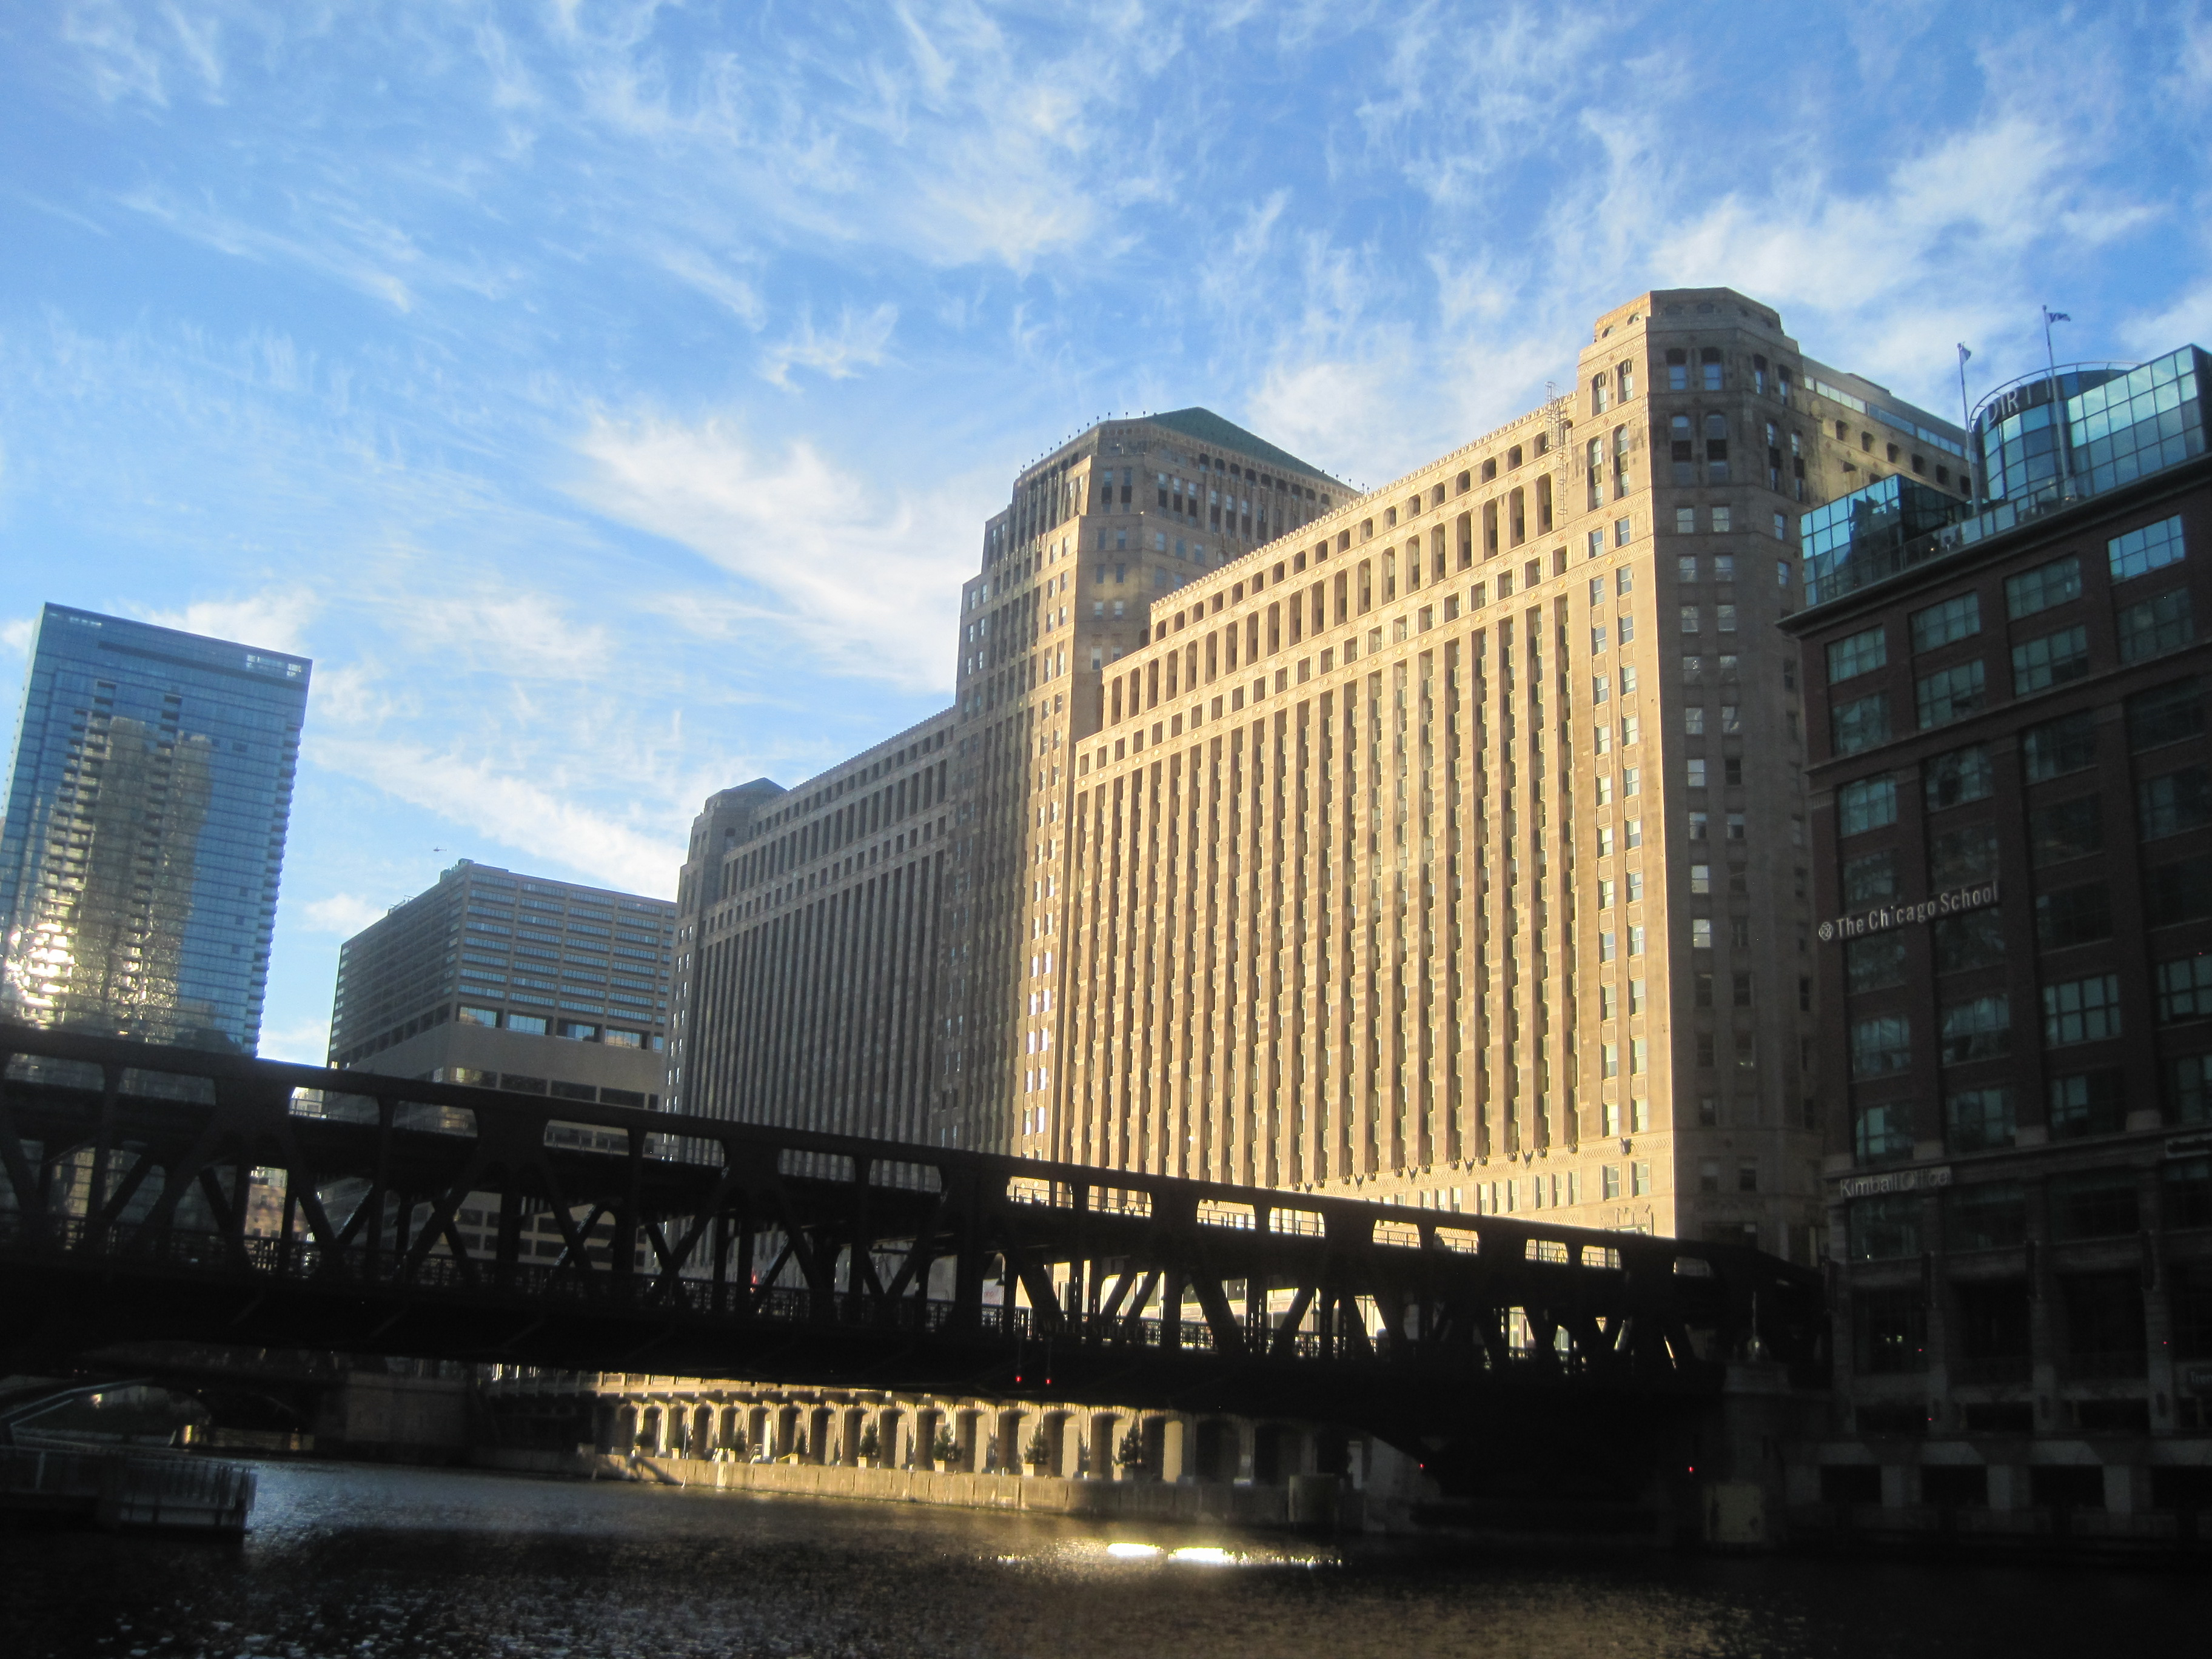
\includegraphics[width=\photosize]{merchmart}}
        
        \uncover<1->{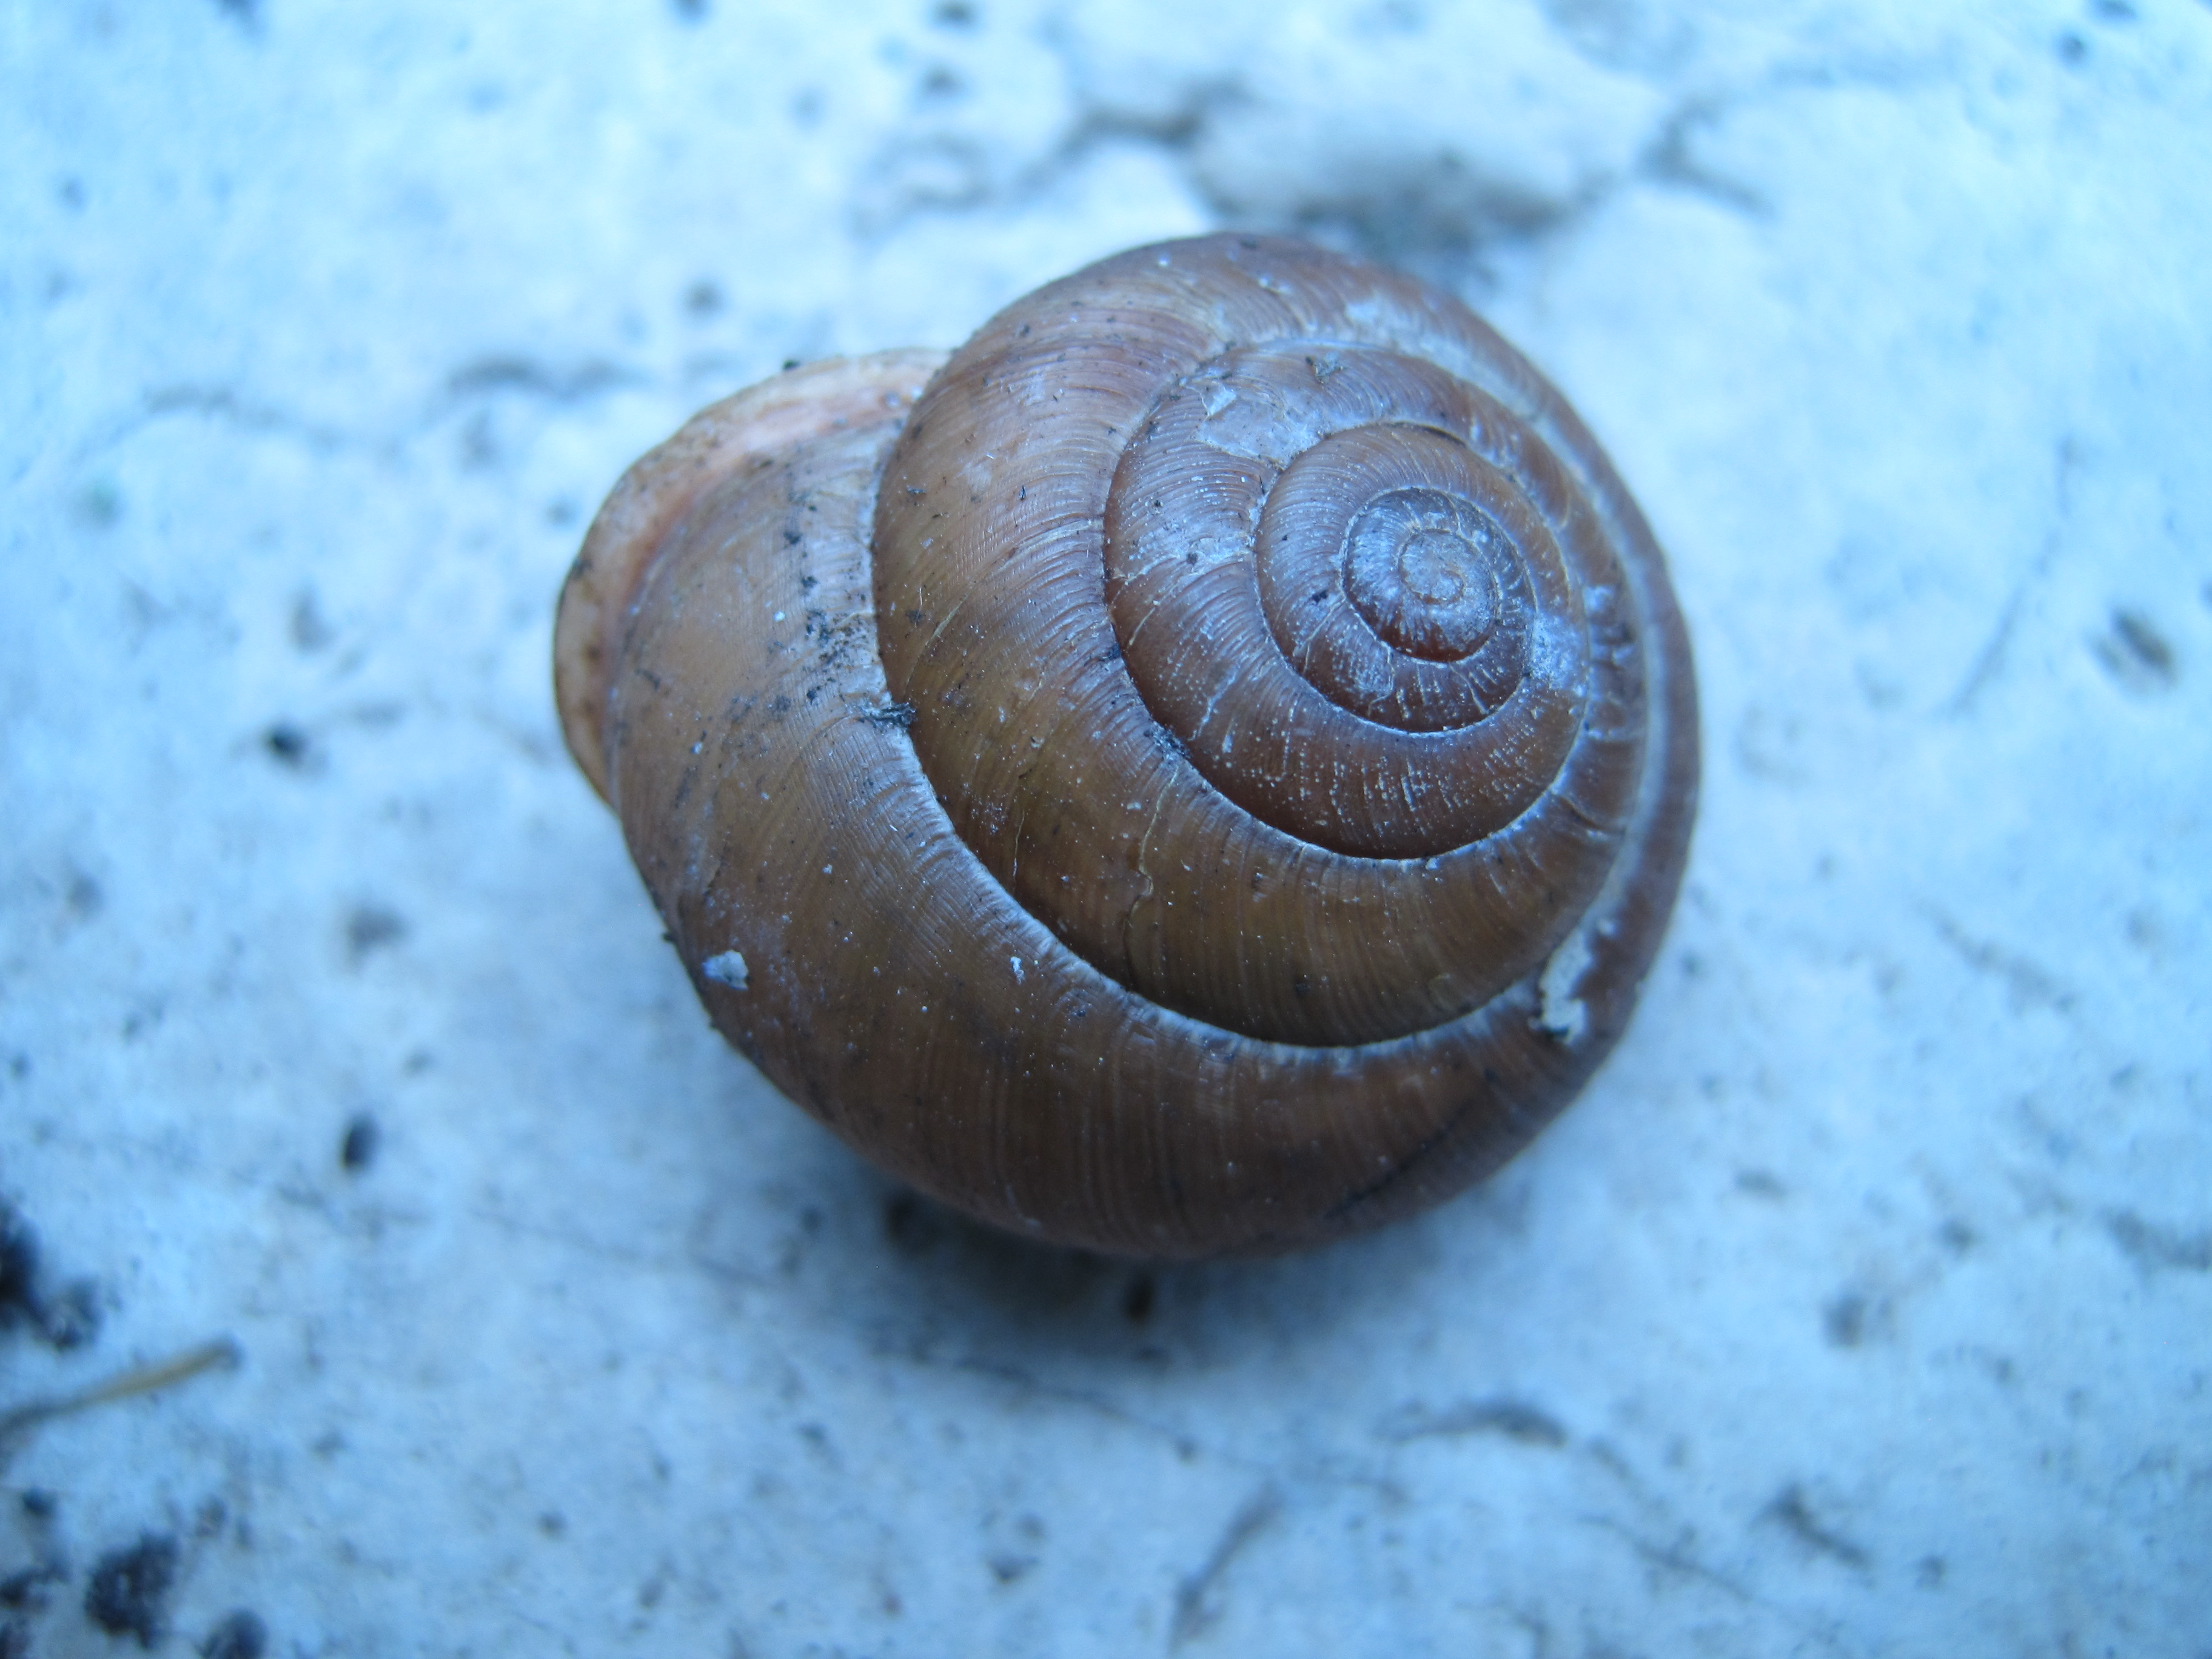
\includegraphics[width=\photosize]{shell}}
        
        \uncover<1, 3->{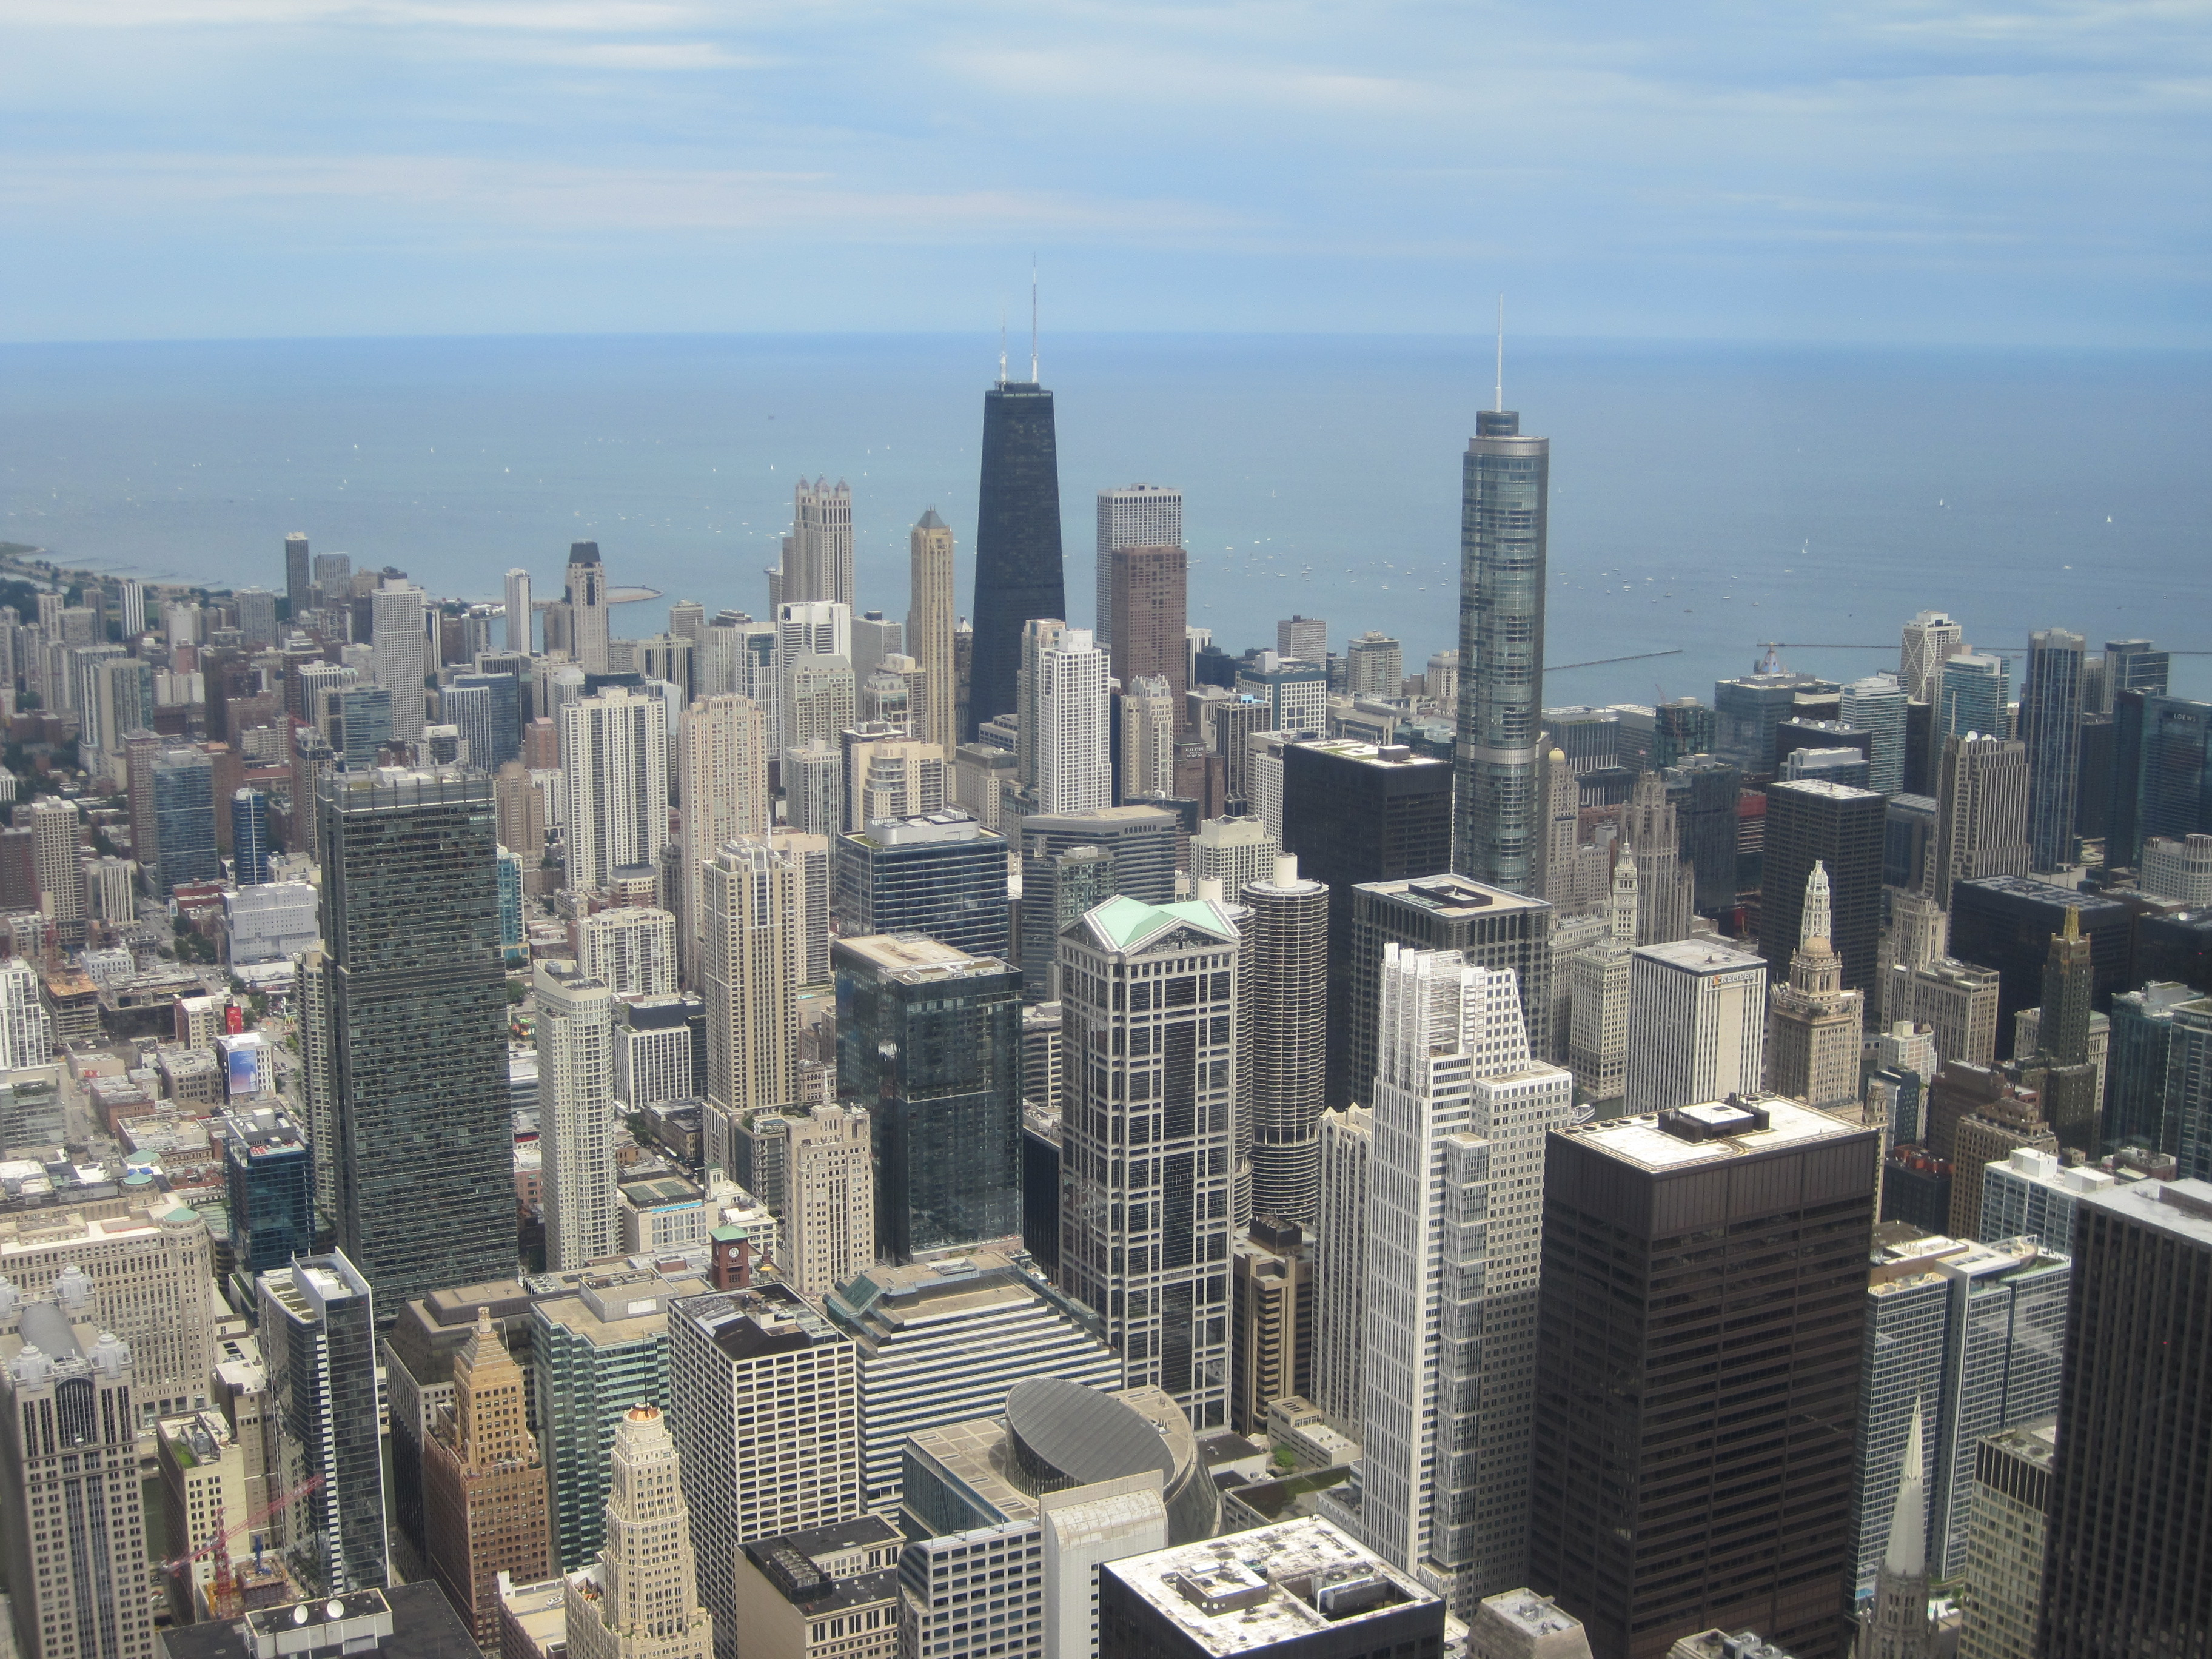
\includegraphics[width=\photosize]{skyline}}
      \end{center}
    \end{column}

    \begin{column}{0.5\textwidth}
      \begin{center}
        \uncover<1->{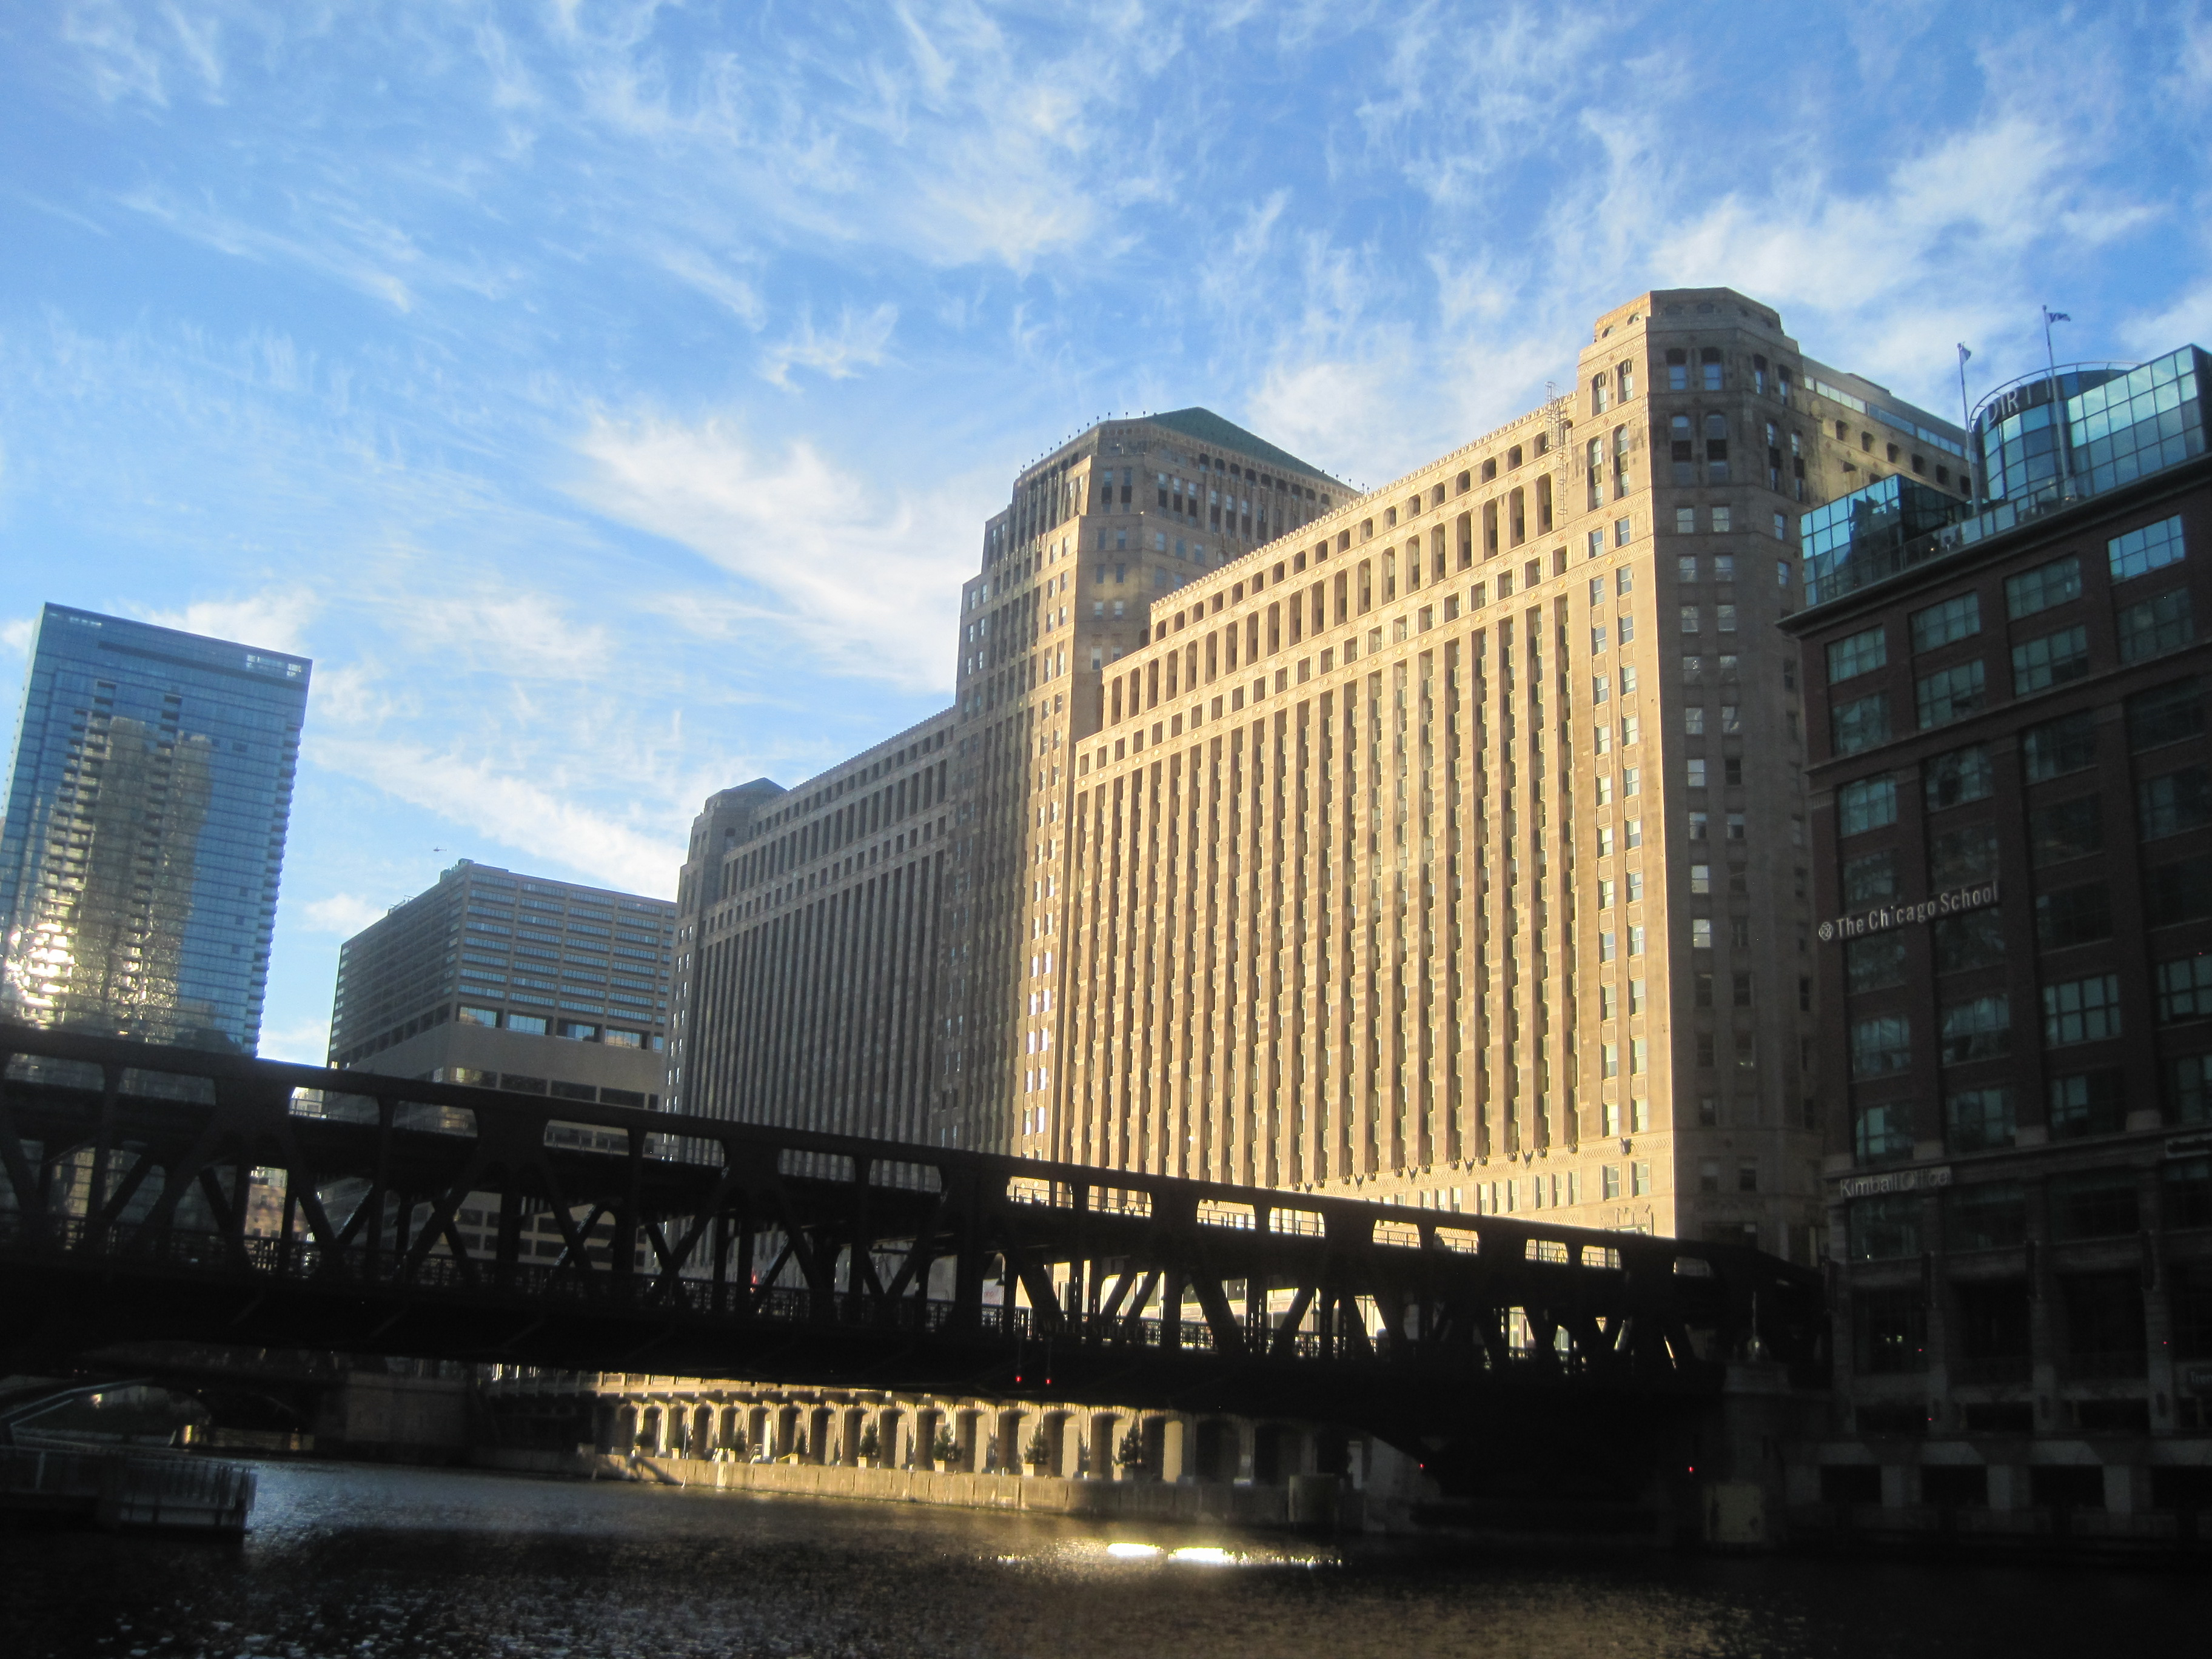
\includegraphics[width=\photosize]{merchmart}}
        
        \uncover<1->{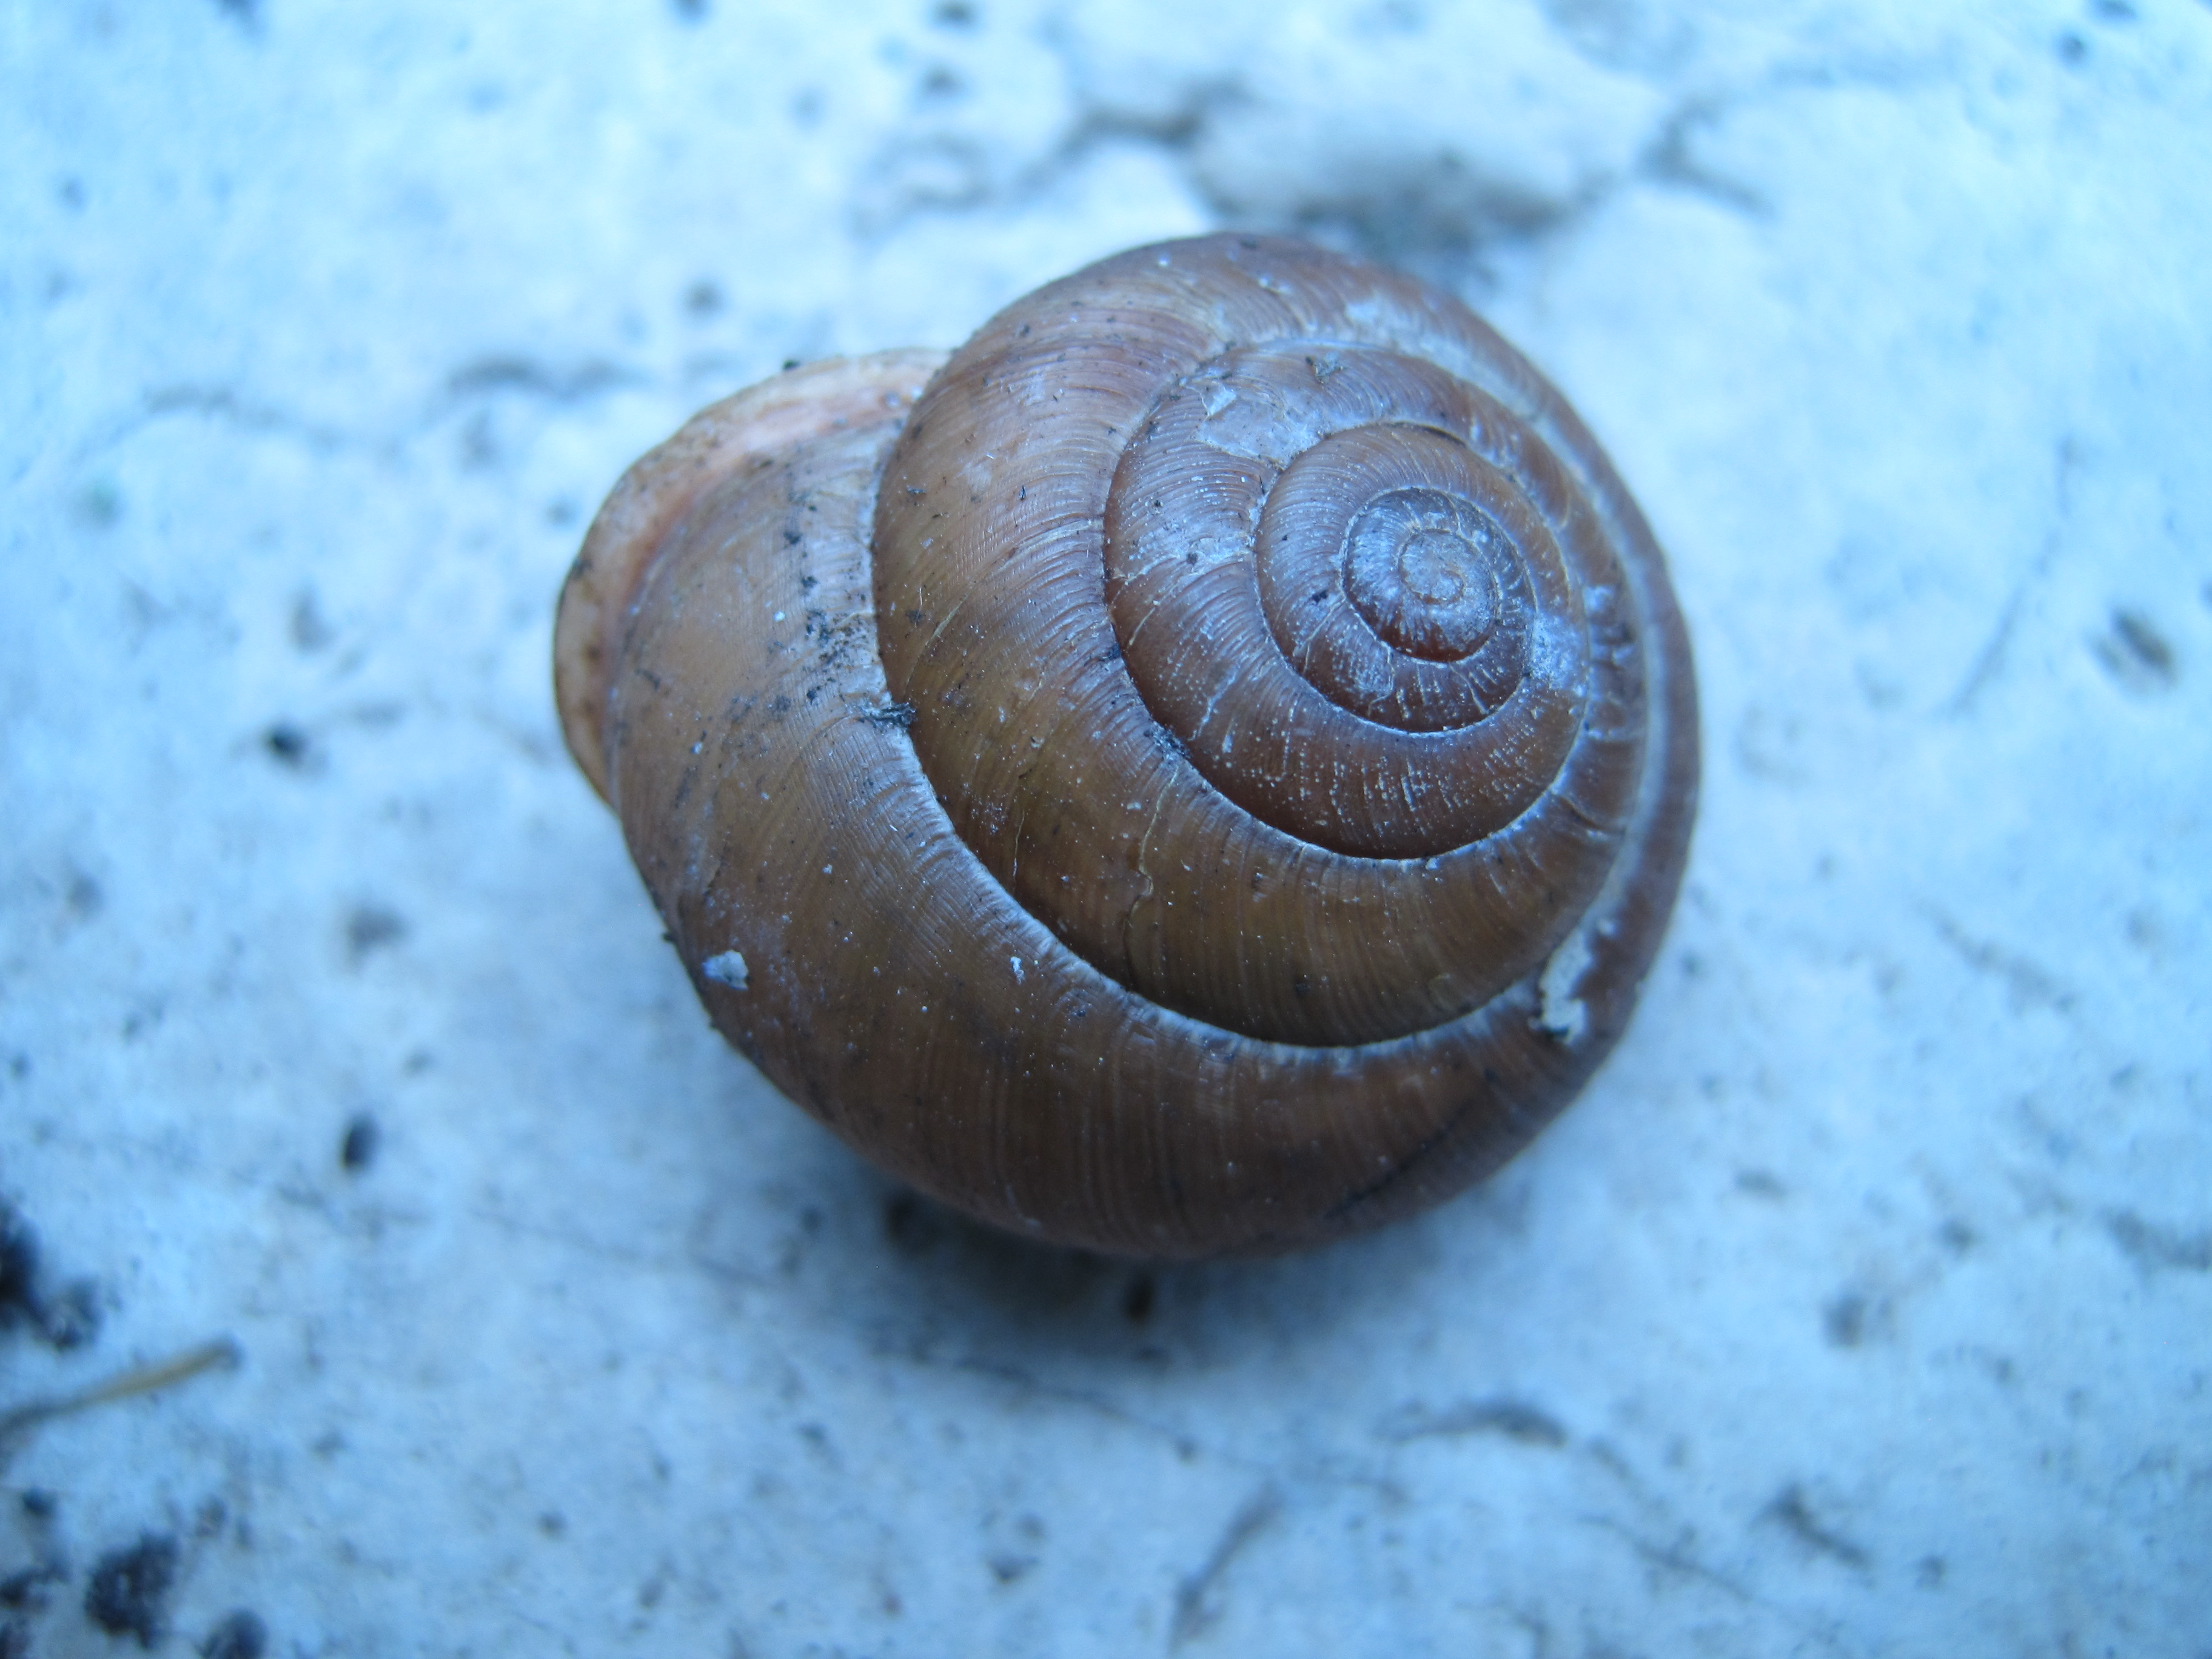
\includegraphics[width=\photosize]{shell}}
        
        \uncover<4->{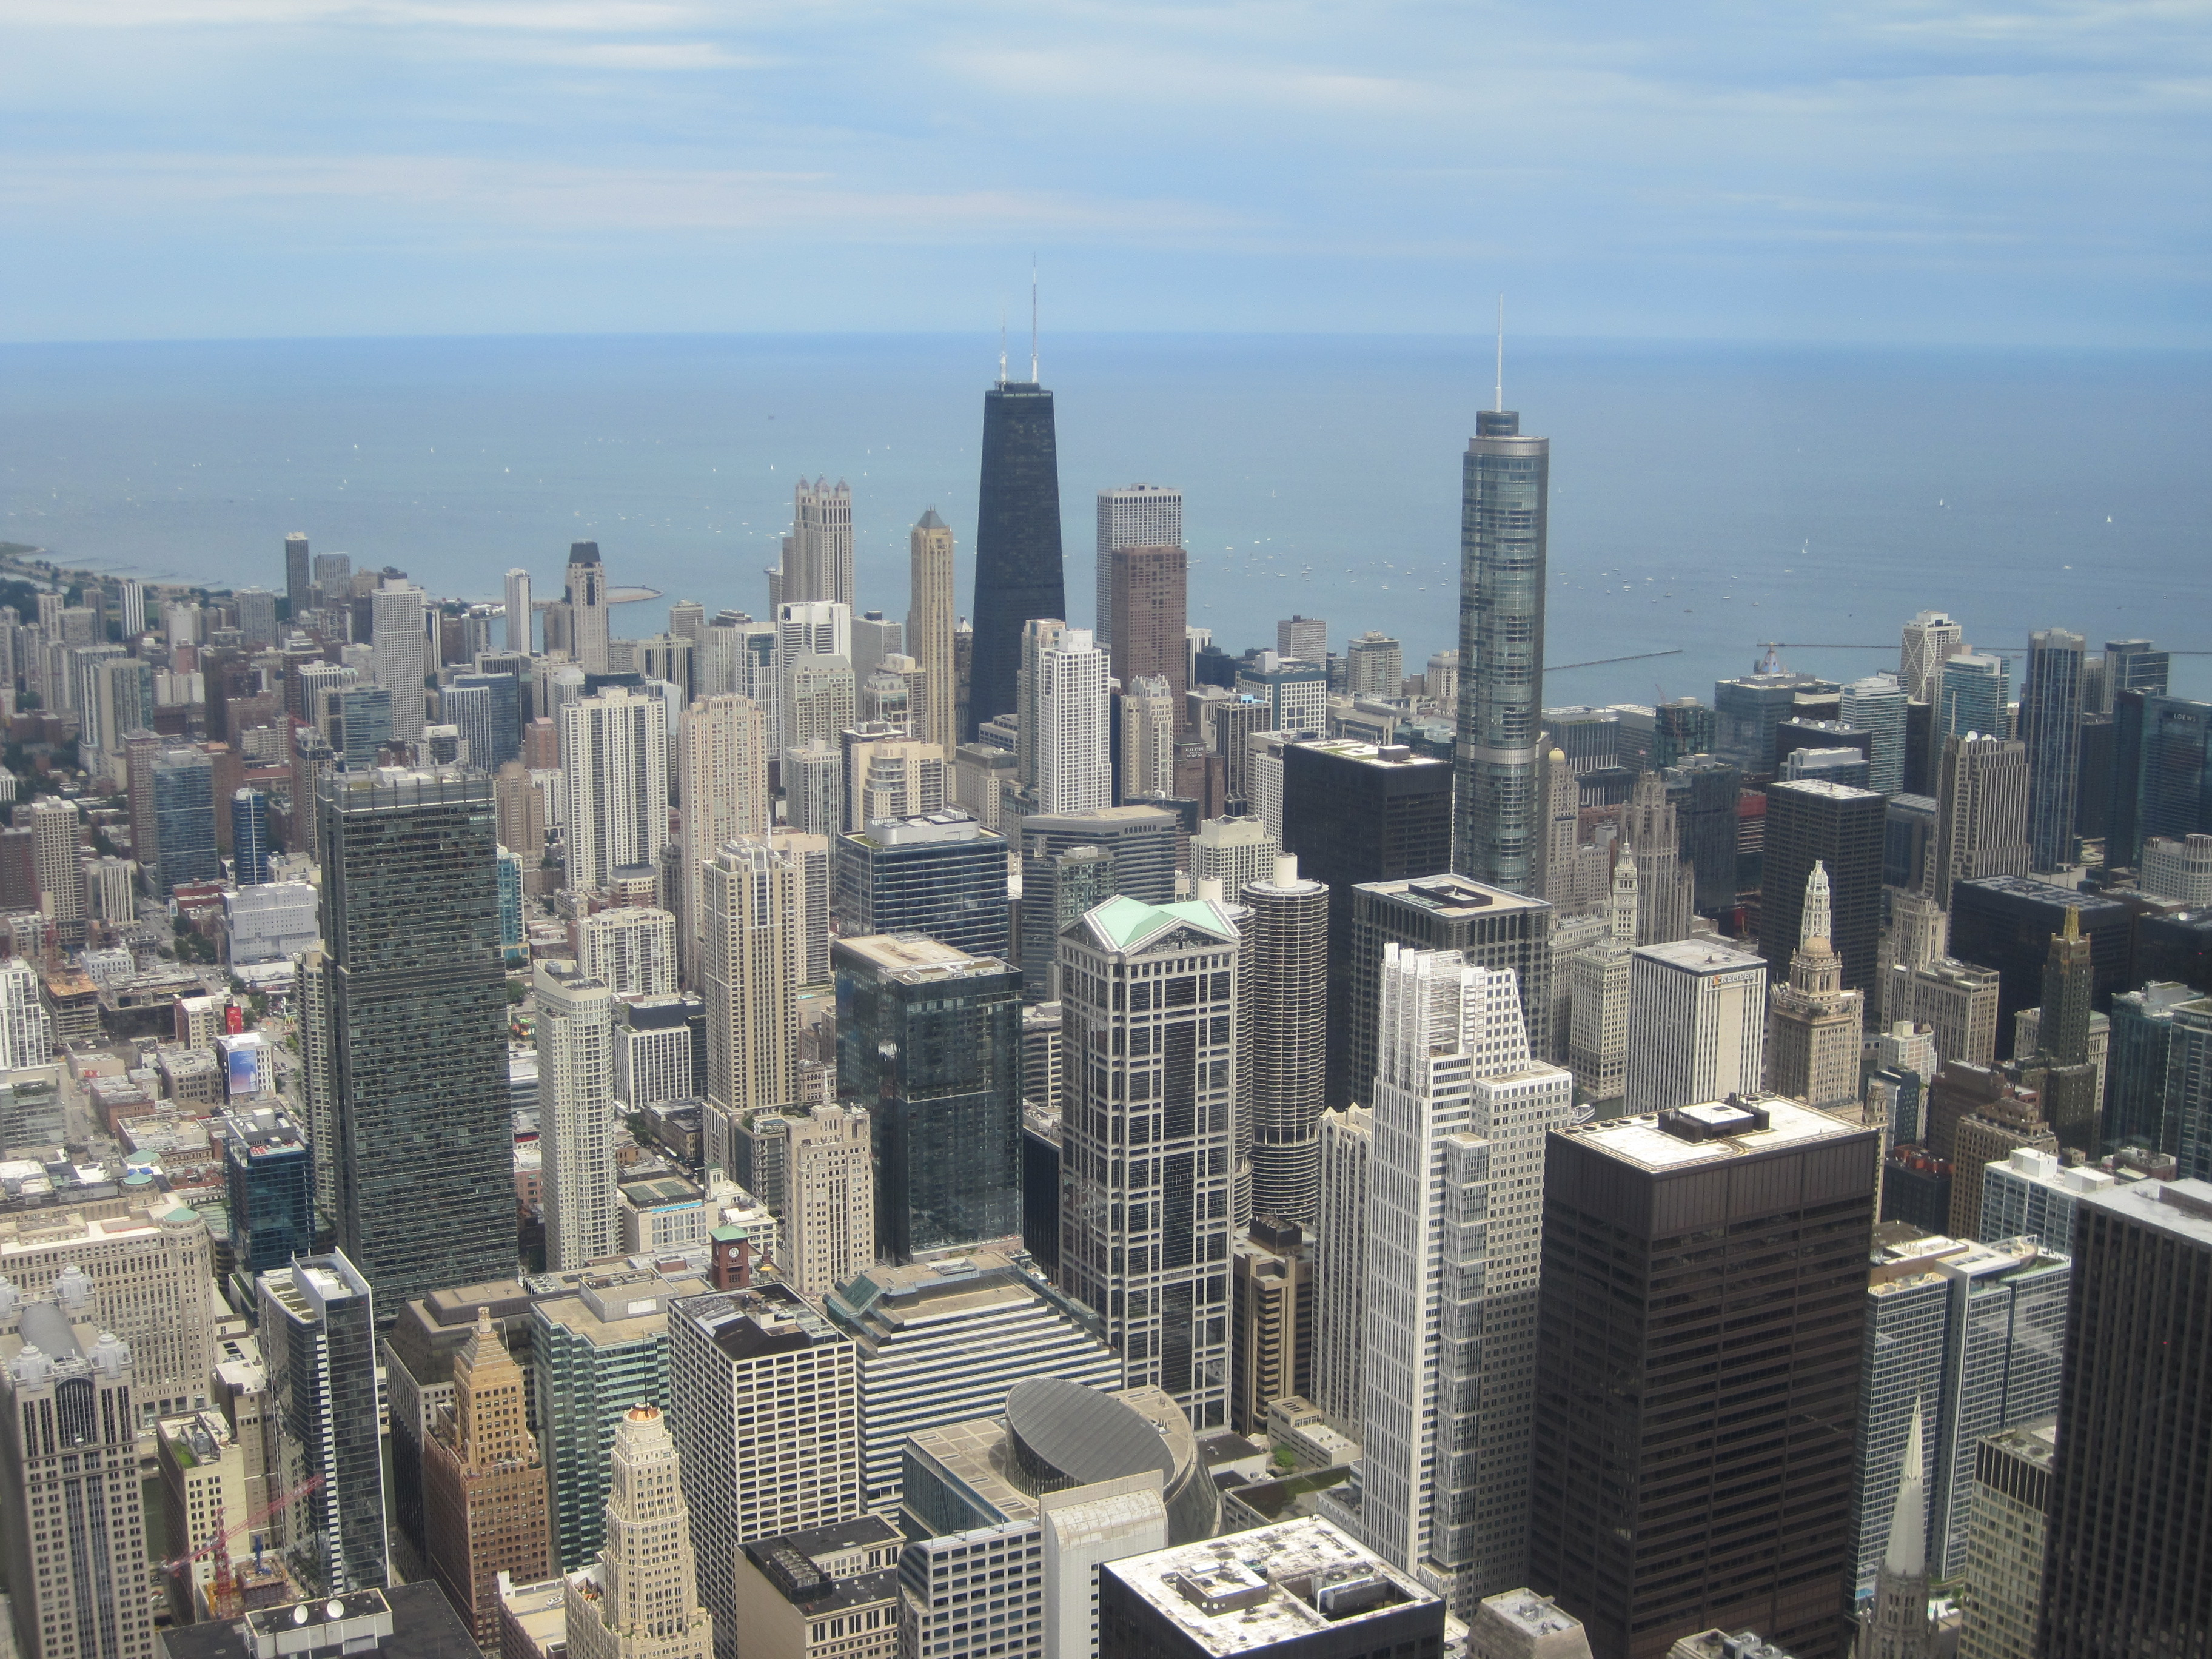
\includegraphics[width=\photosize]{skyline}}
      \end{center}
    \end{column}
  \end{columns}
\end{frame}

\begin{frame}
  \begin{center}
    \begin{tikzpicture}
      \anoncommit{commit1}{(-3, 0)}
      
      \anoncommit{foocommit1}{(-1, 0)}
      \draw (commit1) -- (foocommit1);
      \anoncommit{foocommit2}{(1, 0)}
      \draw (foocommit1) -- (foocommit2);

      \uncover<1-3, 5> {
        \anoncommit{barcommit1}{(-2, 3)}
        \draw (commit1) -- (barcommit1);
        \anoncommit{barcommit2}{(0, 3)}
        \draw (barcommit1) -- (barcommit2);
      }

      \uncover<4-> {
        \anoncommit{rebasebarcommit1}{(2, 3)}
        \draw (foocommit2) -- (rebasebarcommit1);
        \anoncommit{rebasebarcommit2}{(4, 3)}
        \draw (rebasebarcommit1) -- (rebasebarcommit2);
      }
      
      \uncover<2> {
        \anoncommit{mergecommit}{(2, 3)}
        \draw (foocommit2) -- (mergecommit);
        \draw (barcommit2) -- (mergecommit);
      }

      \branch{foo}{(1, 1)}{foo}
      \draw (foo) -- (foocommit2);

      \uncover<1, 3> {
        \branch{bar}{(0, 4)}{bar}
        \draw (bar) -- (barcommit2);
      }

      \uncover<2> {
        \branch{bar}{(2, 4)}{bar}
        \draw (bar) -- (mergecommit);
      }

      \uncover<4-> {
        \branch{bar}{(4, 4)}{bar}
        \draw (bar) -- (rebasebarcommit2);
      }

      \uncover<5> {
        \branch{originbar}{(0, 4)}{origin/bar}
        \draw (originbar) -- (barcommit2);
      }
    \end{tikzpicture}
  \end{center}
\end{frame}

\begin{frame}
  \begin{center}
    \begin{tikzpicture}
      \commit{commit1}{(-4, 0)}{A}
      \uncover<1> { \commit{commit2}{(-2, 0)}{B} }
      \uncover<2-> { \specialcommit{commit2}{(-2, 0)}{E} }
      \draw (commit1) -- (commit2);

      \commit{commit3}{(0, 0)}{C}
      \draw (commit2) -- (commit3);

      \commit{commit4}{(2, 0)}{D}
      \draw (commit3) -- (commit4);

      \uncover<3-> {
        \commit{oldcommit2}{(-3, 3)}{B}
        \draw (commit1) -- (oldcommit2);
        
        \commit{oldcommit3}{(-1, 3)}{C}
        \draw (oldcommit2) -- (oldcommit3);
        
        \commit{oldcommit4}{(1, 3)}{D}
        \draw (oldcommit3) -- (oldcommit4);
      }

      \uncover<4-> {
        \fixupcommit{commit5}{(3, 3)}{F}
        \draw (oldcommit4) -- (commit5);
      }
    \end{tikzpicture}
  \end{center}
\end{frame}

\begin{frame}
  \begin{itemize}
  \item \texttt{git log origin/master...}
  \item \texttt{git diff foo...bar}
  \item \texttt{git add -p}
  \item \texttt{git commit --fixup HEAD~~}
  \item \texttt{git diff origin/bar..}
  \end{itemize}
\end{frame}

\begin{frame}
  \titlepage
\end{frame}

\begin{frame}
  \titlepage
\end{frame}

\end{document}
